% Dokument LaTeX - Analiza spółki Wawel SA (WWL)
\documentclass{article}
\usepackage{graphicx}
\usepackage{polski}
\usepackage[utf8]{inputenc}
\usepackage{amsmath}
\usepackage{array}
\usepackage{amssymb}
\usepackage{hyperref}
\usepackage{float}

\title{Analiza log-zwrotów akcji spółki Wawel SA (WWL)}
\author{Maciej Wojciechowski}
\date{}

\begin{document}

\maketitle

\section{Analiza akcji Wawel SA}

\subsection{Wprowadzenie}
Wawel SA (WWL) jest polskim producentem słodyczy, znanym z produkcji czekolad, cukierków, wafli oraz innych wyrobów cukierniczych. Firma cieszy się długą tradycją na rynku i dostarcza wysokiej jakości produkty konsumentom zarówno w Polsce, jak i za granicą.

Przeprowadzona analiza stanowi pierwszą część projektu zaliczeniowego, w której skupimy się na analizie log-zwrotów akcji spółki Wawel SA.

\subsection{Wykresy kursów zamknięcia oraz log-zwrotów}

\begin{figure}[H]
    \centering
    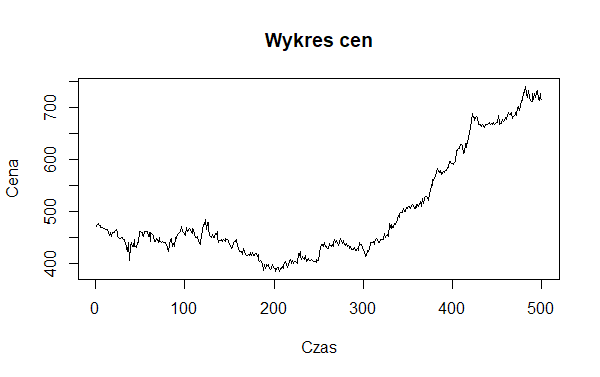
\includegraphics[width=0.8\textwidth]{wykres-cen.png}
    \caption{Wykres cen akcji spółki Wawel SA (WWL)}
    \label{fig:wykres_cen}
\end{figure}

\begin{figure}[H]
    \centering
    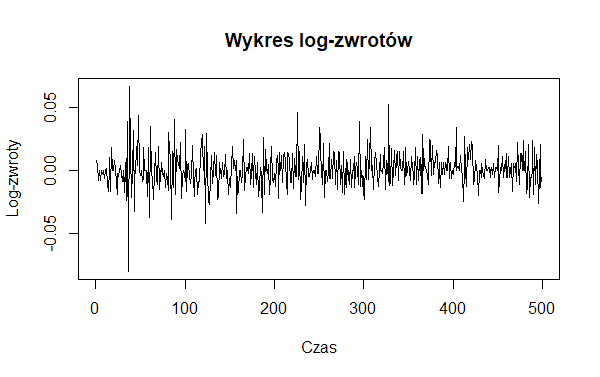
\includegraphics[width=0.8\textwidth]{wykres-log-zwrotow.png}
    \caption{Wykres log-zwrotów akcji spółki Wawel SA (WWL)}
    \label{fig:wykres_log_zwrotow}
\end{figure}

Wykresy powyżej ilustrują zmiany kursów zamknięcia oraz log-zwrotów akcji spółki Wawel SA w czasie. Widać na nich zmienność cen akcji oraz ich wpływ na log-zwroty.

\subsection{Analiza log-zwrotów}
Zakładamy, że log-zwroty $r_1, r_2, \ldots, r_n$ są niezależnymi realizacjami zmiennej losowej $X$ o dystrybuancie $F$, wartości oczekiwanej $\mu$ i wariancji $\sigma^2$. 

Odpowiednie estymatory użyte w analizie to:
\begin{equation}
    \hat{\mu} = \frac{1}{n} \sum_{i=1}^{n} r_i
\end{equation}
\begin{equation}
    \hat{\sigma}^2 = \frac{1}{n-1} \sum_{i=1}^{n} (r_i - \hat{\mu})^2
\end{equation}
\begin{equation}
    \hat{\sigma} = \sqrt{\hat{\sigma}^2}
\end{equation}

Korzystając z klasycznego estymatora kwantyli, wyestymowano kwantyle rzędu $\alpha = 5\%, 50\%, 95\%$. Wyniki zostały przedstawione w tabeli poniżej:

\begin{table}[H]
    \centering
    \begin{tabular}{|l|r|}
        \hline
        \textbf{Estymator} & \textbf{Wartość} \\
        \hline
        Liczność próby ($n$) & 499 \\
        Wartość oczekiwana ($\hat{\mu}$) & 0,000837 \\
        Wariancja ($\hat{\sigma}^2$) & 0,000202 \\
        Odchylenie standardowe ($\hat{\sigma}$) & 0,014220 \\
        Kwantyl 5\% ($q_{5\%}$) & -0,020416 \\
        Kwantyl 50\% ($q_{50\%}$) & 0,000000 \\
        Kwantyl 95\% ($q_{95\%}$) & 0,023786 \\
        \hline
    \end{tabular}
    \caption{Podstawowe statystyki log-zwrotów akcji spółki Wawel SA (WWL)}
    \label{tab:wyniki}
\end{table}

\begin{figure}[H]
    \centering
    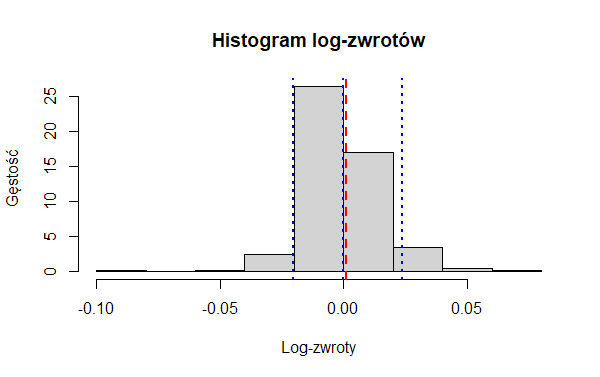
\includegraphics[width=0.8\textwidth]{histogram-log-zwrotow.png}
    \caption{Histogram log-zwrotów z zaznaczoną średnią i kwantylami}
    \label{fig:histogram_log_zwrotow}
\end{figure}

\subsection{Interpretacja kwantyli}
Każdy z kwantyli ma swoją specyficzną interpretację w kontekście log-zwrotów akcji:
\begin{itemize}
    \item \textbf{Kwantyl 5\%}: Wartość log-zwrotu, poniżej której znajduje się 5\% najmniejszych obserwacji. Oznacza to, że istnieje 5\% szans, że log-zwrot będzie niższy niż -0,020416.
    \item \textbf{Kwantyl 50\% (mediana)}: Wartość środkowa log-zwrotów. Oznacza to, że połowa log-zwrotów jest większa, a połowa mniejsza niż 0,000000.
    \item \textbf{Kwantyl 95\%}: Wartość log-zwrotu, poniżej której znajduje się 95\% obserwacji. Oznacza to, że tylko 5\% log-zwrotów jest wyższych niż 0,023786.
\end{itemize}

\subsection{Estymacja dystrybuanty}
W celu estymacji dystrybuanty $F$ wykorzystano empiryczny estymator dystrybuanty, którego wzór jest następujący:
\begin{equation}
    \hat{F}(x) = \frac{1}{n} \sum_{i=1}^{n} I(r_i \leq x),
\end{equation}
 gdzie $I(r_i \leq x)$ jest funkcją indykatora, a $n$ oznacza liczbę obserwacji.

Dystrybuanta empiryczna została przedstawiona na wykresie poniżej:

\begin{figure}[H]
    \centering
    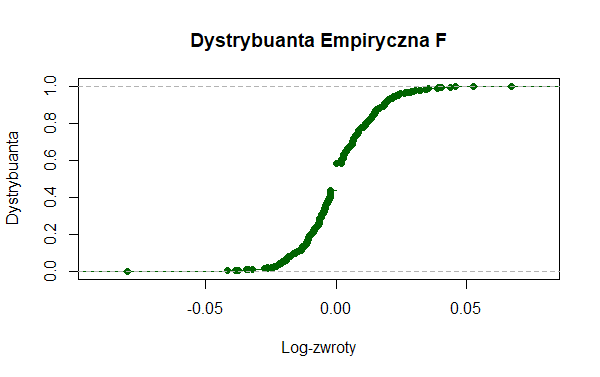
\includegraphics[width=0.8\textwidth]{dystrybuanta-empiryczna.png}
    \caption{Dystrybuanta empiryczna $\hat{F}(x)$ dla log-zwrotów}
    \label{fig:dystrybuanta_empiryczna}
\end{figure}

\section{Analiza dobroci dopasowania rozkładu normalnego i t-Studenta}

\subsection{Estymacja parametrów}

Wykorzystując estymator największej wiarygodności (MLE) oraz bibliotekę \texttt{fitdistrplus} w R, wyestymowano parametry rozkładu normalnego i t-Studenta dla danych log-zwrotów.

\subsubsection{Rozkład normalny}

\begin{table}[H]
    \centering
    \begin{tabular}{|l|r|r|}
        \hline
        & \textbf{Estymata} & \textbf{Błąd standardowy} \\
        \hline
        Średnia ($\hat{\mu}$) & 0,000837 & 0,000636 \\
        Odchylenie standardowe ($\hat{\sigma}$) & 0,014205 & 0,000440 \\
        \hline
    \end{tabular}
    \caption{Estymowane parametry rozkładu normalnego}
    \label{tab:fit_norm}
\end{table}

\subsubsection{Rozkład t-Studenta}

\begin{table}[H]
    \centering
    \begin{tabular}{|l|r|r|}
        \hline
        & \textbf{Estymata} & \textbf{Błąd standardowy} \\
        \hline
        Liczba stopni swobody ($\hat{\nu}$) & 4,9764 & 1,1504 \\
        Średnia ($\hat{\mu}$) & 0,000344 & 0,000578 \\
        Skala ($\hat{\sigma}$) & 0,011042 & 0,000611 \\
        \hline
    \end{tabular}
    \caption{Estymowane parametry rozkładu t-Studenta}
    \label{tab:fit_t}
\end{table}

\subsection{Wykresy diagnostyczne}

\subsubsection{Histogram z nałożonymi gęstościami}

\begin{figure}[H]
    \centering
    \includegraphics[width=0.8\textwidth]{histogram_z_gestosciami.png}
    \caption{Histogram log-zwrotów z nałożonymi funkcjami gęstości rozkładów normalnego i t-Studenta}
    \label{fig:histogram_gestosci}
\end{figure}

\textbf{Opis:} Wykres histogramu przedstawia empiryczny rozkład danych, na który nałożono dopasowane gęstości rozkładów normalnego (niebieska linia) i t-Studenta (czerwona linia przerywana).  
Analiza wykazuje, że:
\begin{itemize}
    \item Rozkład normalny (niebieski) lepiej odwzorowuje dane empiryczne, szczególnie w centralnym zakresie wartości.
    \item Rozkład t-Studenta (czerwony) jest znacząco niedopasowany.
\end{itemize}

\subsubsection{Wykres kwantyl-kwantyl (Q-Q plot)}

\begin{figure}[H]
    \centering
    \includegraphics[width=0.8\textwidth]{wykres-qq.png}
    \caption{Wykres Q-Q dla rozkładów normalnego i t-Studenta}
    \label{fig:qq_plot}
\end{figure}

\textbf{Opis:} Wykres QQ porównuje kwantyle empiryczne danych z kwantylami teoretycznymi rozkładów normalnego i t-Studenta.  
Na wykresie zauważalne są następujące cechy:
\begin{itemize}
    \item Punkty dla rozkładu normalnego (niebieskie) układają się niemal idealnie wzdłuż linii prostej, co sugeruje wysoką zgodność z danymi empirycznymi.
    \item Rozkład t-Studenta (czerwony) znacznie odstaje od linii prostej, wskazując na niedopasowanie tego rozkładu do danych.
\end{itemize}

\subsubsection{Porównanie dystrybuant (CDF)}

\begin{figure}[H]
    \centering
    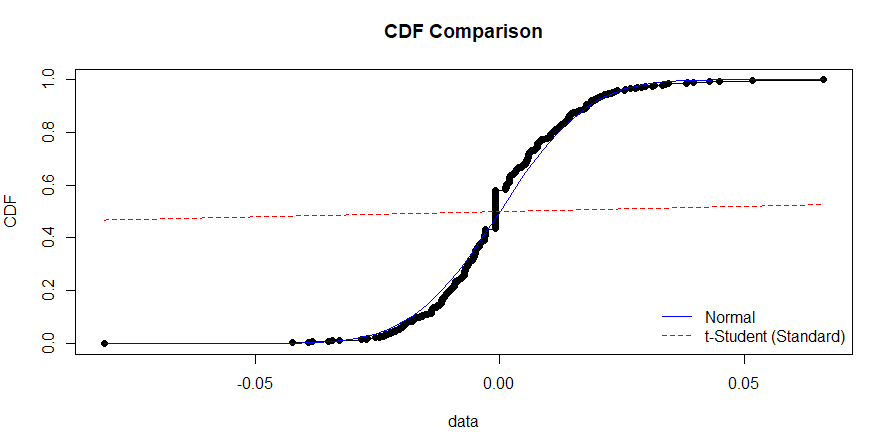
\includegraphics[width=0.8\textwidth]{dystrybuanta-empiryczna-vs-teoretyczna.png}
    \caption{Porównanie dystrybuant empirycznej z teoretycznymi dla rozkładów normalnego i t-Studenta}
    \label{fig:dystrybuanta_vs_teoretyczna}
\end{figure}

\textbf{Opis:} Wykres porównuje empiryczną dystrybuantę danych z teoretycznymi dystrybuantami rozkładów normalnego i t-Studenta.  
Główne obserwacje:
\begin{itemize}
    \item Dystrybuanta rozkładu normalnego (niebieska linia) doskonale pokrywa się z empiryczną dystrybuantą danych.
    \item Dystrybuanta rozkładu t-Studenta (czerwona linia przerywana) wykazuje znaczne rozbieżności, co wskazuje na niedopasowanie.
\end{itemize}

\subsubsection{Wykres P-P (Probability-Probability plot)}

\begin{figure}[H]
    \centering
    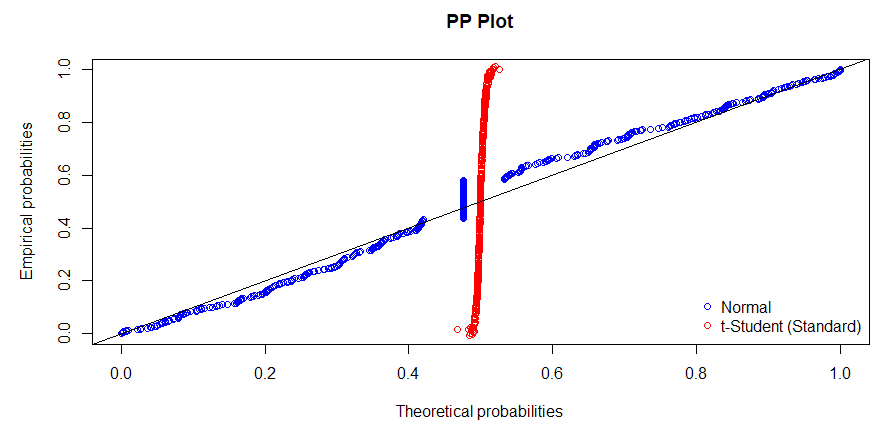
\includegraphics[width=0.8\textwidth]{wykres-pp.png}
    \caption{Wykres P-P dla rozkładów normalnego i t-Studenta}
    \label{fig:pp_plot}
\end{figure}

\textbf{Opis:} Wykres PP ilustruje zgodność empirycznych prawdopodobieństw z teoretycznymi dla rozkładu normalnego. Natomiast dane rozkładu T-Studenta znacząco odbiegają od danych rzeczywistych.  
Z analizy wynika:
\begin{itemize}
    \item Punkty dla rozkładu normalnego (niebieskie) układają się niemal idealnie wzdłuż linii przekątnej, co potwierdza bardzo dobre dopasowanie do danych.
    \item Rozkład t-Studenta (czerwony) pokazuje znaczne odstępstwa od linii przekątnej, co sugeruje istotne niedopasowanie.
\end{itemize}

\subsection{Ocena dopasowania rozkładów}

Analiza jednoznacznie wskazuje, że dane empiryczne są znacznie lepiej modelowane przez rozkład \textbf{normalny} niż przez rozkład t-Studenta.  
\textbf{Wnioski:}
\begin{itemize}
    \item Rozkład normalny charakteryzuje się bliskim dopasowaniem zarówno w centralnej części, jak i w ogonach.
    \item Rozkład t-Studenta znacząco odbiega od danych, co czyni go nieodpowiednim w tym przypadku.
\end{itemize}

\subsection*{Interpretacja statystyk dopasowania rozkładów}

\subsection*{Statystyki dopasowania (\textit{Goodness-of-fit statistics})}

\begin{table}[h!]
\centering
\begin{tabular}{|l|c|c|}
\hline
\textbf{Statystyka}            & \textbf{Normalny} & \textbf{t-Studenta} \\ \hline
Kolmogorov-Smirnov             & 0.1047            & 0.4811             \\ \hline
Cramer-von Mises               & 0.6771            & 40.0829            \\ \hline
Anderson-Darling               & 3.5170            & 186.7583           \\ \hline
\end{tabular}
\caption{Porównanie statystyk dopasowania rozkładów}
\end{table}

\textbf{Interpretacja:}
\begin{itemize}
    \item Rozkład normalny uzyskał znacznie niższe wartości dla wszystkich trzech statystyk, co wskazuje na lepsze dopasowanie do danych w porównaniu z rozkładem t-Studenta.
    \item Szczególnie wartość statystyki Andersona-Darlinga dla rozkładu t-Studenta ($186.7583$) podkreśla jego niedopasowanie.
\end{itemize}

\subsection*{Kryteria dopasowania (\textit{Goodness-of-fit criteria})}

\begin{table}[h!]
\centering
\begin{tabular}{|l|c|c|}
\hline
\textbf{Kryterium}                     & \textbf{Normalny} & \textbf{t-Studenta} \\ \hline
Akaike's Information Criterion (AIC)  & -2825.534         & 919.8094            \\ \hline
Bayesian Information Criterion (BIC)  & -2817.109         & 924.0220            \\ \hline
\end{tabular}
\caption{Porównanie kryteriów dopasowania rozkładów}
\end{table}

\textbf{Interpretacja:}
\begin{itemize}
    \item Zarówno kryterium Akaike'go (AIC), jak i kryterium Bayesowskie (BIC) wskazują, że rozkład normalny jest znacznie lepiej dopasowany niż rozkład t-Studenta.
    \item Niższe wartości dla rozkładu normalnego ($-2825.534$ dla AIC oraz $-2817.109$ dla BIC) wskazują na przewagę tego modelu w uwzględnianiu dopasowania i prostoty modelu.
\end{itemize}

\subsection*{Podsumowanie}

Na podstawie przedstawionych statystyk i kryteriów dopasowania:
\begin{itemize}
    \item Rozkład \textbf{normalny} jest znacznie lepszy w modelowaniu danych niż rozkład t-Studenta.
    \item Rozkład t-Studenta charakteryzuje się dużymi odstępstwami w dopasowaniu, co czyni go nieodpowiednim w tym przypadku.
\end{itemize}



\subsection{Test hipotezy metodą Monte Carlo}

Dla wybranego rozkładu t-Studenta przeprowadzono test hipotezy o równości rozkładów, wykorzystując statystykę Kolmogorowa-Smirnowa (KS) oraz metodę Monte Carlo. Wyniki testu przedstawiono w tabeli 5.

\begin{table}[H]
    \centering
    \begin{tabular}{|p{7cm}|c|}
        \hline
        \textbf{Wynik} & \textbf{Wartość} \\
        \hline
        Zaobserwowana statystyka KS & 0,0893735 \\
        P-wartość z symulacji Monte Carlo & 0 \\
        \hline
    \end{tabular}
    \caption{Wyniki testu hipotezy metodą Monte Carlo}
    \label{tab:test_results}
\end{table}


\textbf{Interpretacja:} P-wartość równa 0 wskazuje na silne podstawy do odrzucenia hipotezy zerowej, że dane pochodzą z rozkładu t-Studenta z wyestymowanymi parametrami. Oznacza to, że mimo lepszego dopasowania w porównaniu z rozkładem normalnym, rozkład t-Studenta nie jest w stanie w pełni opisać danych log-zwrotów.

\section*{Histogram logarytmicznych zwrotów}

\textbf{Opis:} Histogram przedstawia empiryczny rozkład logarytmicznych zwrotów danych:

\begin{figure}[H]
    \centering
    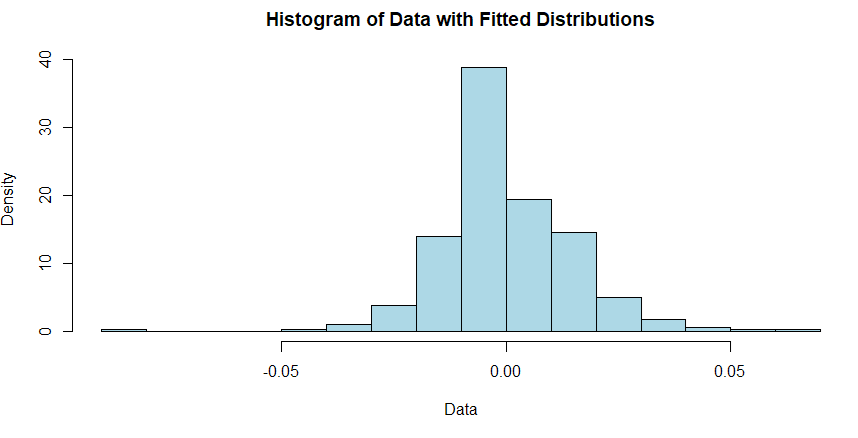
\includegraphics[width=0.8\textwidth]{histogram_log_returns.png}
    \caption{Histogram logarytmicznych zwrotów}
    \label{fig:histogram_log_returns}
\end{figure}

\section{Podsumowanie}

Przeprowadzona analiza log-zwrotów akcji spółki Wawel SA wykazała, że:

\begin{itemize}
    \item Średnia log-zwrotów jest bliska zeru, co sugeruje brak wyraźnego trendu wzrostowego lub spadkowego w badanym okresie.
    \item Odchylenie standardowe wskazuje na umiarkowaną zmienność log-zwrotów.
    \item Kwantyle pokazują asymetrię w rozkładzie log-zwrotów, co jest typowe dla danych finansowych.
    \item Rozkład normalny lepiej dopasowuje się do danych niż rozkład T-Studenta, co potwierdzają statystyki dobroci dopasowania i kryteria informacyjne.
    \item Test hipotezy metodą Monte Carlo sugeruje odrzucenie hipotezy, że dane pochodzą z rozkładu t-Studenta, wskazując na lepsze dopasowanie wyników otrzymanych z rozkładu normalnego.
\end{itemize}

\end{document}